\section*{3. Logistic Regression 1}
Discriminative model, because it models the posterior probabilities $p(y|x)$ directly.         

\subsection*{Posteriors and the Logistic Function}
\begin{itemize}
    \item
        For two classes $y \in \{0,1\}$ we get:\\
        \begin{align*}
        p(y=0|x) &= \ffrac{p(y=0) \cdot p(x|y=0)}{p(x)} 
        = \ffrac{p(y=0) \cdot p(x|y=0)}{p(y=0)p(x|y=0) + p(y=1)p(x|y=1)} 
        = \ffrac{1}{1+ \ffrac{p(y=1)p(x|y=1)}{p(y=0)p(x|y=0)}}\\
        &= \ffrac{1}{1+ e^{log\ffrac{p(y=1)p(x|y=1)}{p(y=0)p(x|y=0)}}}
        = \ffrac{1}{1+ e^{-log\ffrac{p(y=0)}{p(y=1)} - log\ffrac{p(x|y=0)}{p(x|y=1)}}}
        \end{align*}
    \item
        We see that the posteriors can be written in terms of a logistic funtion\\
        $p(y=0|x) = \ffrac{1}{1+e^{-F(x)}}$\\
        with\\
        $p(y=1|x) = 1-p(y=0|x) = \dots = \ffrac{1}{1+e^{F(x)}}$
    \item
        The logistic function (also called sigmoid function) is defined by
        $g(x) = \ffrac{1}{1+e^{-x}}, x \in \mathbb{R}$
    \item
        The derivative has the nice property $g'(x) = \dots = g(x)g(-x) = g(x)(1-g(x))$
        \begin{figure}[H]
            \centering
            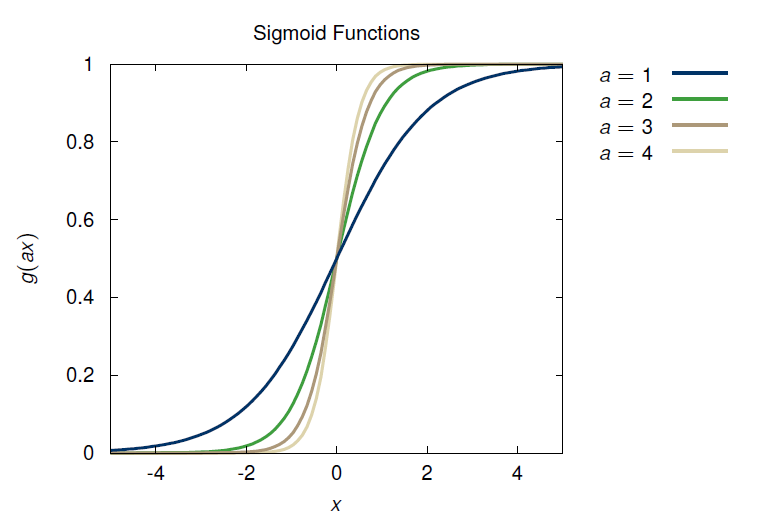
\includegraphics[width=0.5\textwidth]{figures/pr03_3-8}
            \caption{Sigmoid function $g(ax) = 1/(1 + e^{-ax}) for a = 1,2,3,4$}
        \end{figure}
\end{itemize}
\subsection*{Decision boundary}
\begin{itemize}
    \item
        Decision boundary $\delta(x) = 0$ seperates two classes: \\
        $p(y=0|x) = p(y=1|x)$ and thus $log \ffrac{p(y=0|x)}{p(y=1|x)} = log 1 = 0$
    \item
        One can show that decision boundary is given by $F(x) = 0$ by starting with\\
        $log \ffrac{p(y=0|x)}{p(y=1|x)} = F(x) = 0$
    \item
        If class-conditionals are Gaussian and they both share the same covariance matrix, the decision boundary is linear        
    \item
        If all class-conditional densities are members of the same exponential family of pdfs with equal dispersion $\phi$, the decision boundary $F(x) = 0$ is linear in the components of x
    \item
        The exponential family is a class of pdf's that can be written in the following canonical form\\
        $p(x, \Theta, \phi) = e^{\ffrac{\Theta^T \cdot x - b(\Theta)}{a(\phi)} + c(x, \phi)}$\\
        where $\Theta \in \mathbb{R}^d$ is the location parameter vector, $\phi$ the dispersion parameter.
    \item
        Exampels are Gaussian pdf, Exponential pdf, Binomial Probability Mass Function, Poisson Probability Mass Function and Hypergeometric Probability Mass Function
\end{itemize}
